\chapter{Transport domain formulation}

In this chapter, we will formalize variants of the Transport domain and mention a few related transportation problems that have been studied in the past.

\section{Description of Transport domain variants}

Transport is a planning domain designed for
the International Planning
Competition\footnote{\url{http://www.icaps-conference.org/index.php/Main/Competitions}}
(IPC), which is part of the International Conference on Automated Planning and
Scheduling\footnote{\url{http://www.icaps-conference.org/index.php/Main/HomePage}} (ICAPS).
Originally, Transport appeared at 
IPC-6\footnote{\url{http://icaps-conference.org/ipc2008/deterministic/Domains.html}} which took place in 2008.
Since then, it has been used in two IPCs,
specifically IPC-7\footnote{\url{http://www.plg.inf.uc3m.es/ipc2011-deterministic/}} in 2011
and IPC-8\footnote{\url{https://helios.hud.ac.uk/scommv/IPC-14/}} in 2014.

There are a few basic formulations of the Transport domain family (i.e.~``similar'' Transport domain variants) which we will describe in the following sections. One variant which we will not study
in this work is the NoMystery domain from IPC 2011,
devised as a simplification of Transport (using only a single
vehicle with no capacity constraints).
The domain assumes
fuel costs for driving on roads, with the vehicle
having an initial fuel capacity (there is no refueling).
All actions have a cost of 1.
It is reasonably straightforward to solve problems of this variant using domain-specific knowledge as shown in \citet{Bartak2016}: the vehicle is always greedily loaded
with all the packages present at a location when arriving at it and
greedily unloaded when it contains a package which has the given location as a destination. Choosing which roads the vehicle drives
along and thus determining
the order of package loading and unloading 
while taking into account the fuel constraints is
the task that is left for the planner to solve.

\subsection{Common traits of Transport domains}

Transport is a logistics domain --- vehicles drive around on a (generally asymmetric) positively-weighted oriented graph, picking up and dropping packages along the way.
All vehicles have limited capacities (the sum of package sizes they can carry).
Picking up or dropping a package costs 1 unit. The cost of driving along a road is equal to the edge weight
(in other words, the road length).
The general goal is to minimize the \textit{total cost}
while delivering all packages to their destination, where
the total cost of a plan is defined as the sum of the costs of all actions in
the plan.

A few Transport problems also request that the vehicles be positioned at certain
locations in the graph
after finishing their deliveries.

\subsection{Transport STRIPS}\label{transport-strips}

STRIPS, the Stanford Research Institute Problem Solver,
was a planner proposed in the 1970s by \citet{Fikes1971}.
The influence of STRIPS was, however, not only due to the planner,
but the language used to describe its inputs --- the planning operators and goals.
That is why we sometimes refer to classical planning (Section~\ref{classical-planning})
as STRIPS planning. For the purposes of this text, we will use these terms interchangeably.

In the STRIPS variant of the Transport domain,
all packages have a size of 1 and vehicles of a bounded capacity can drive around indefinitely
(there is no notion of fuel or anything similar). The only reason for them not to, is that
driving incurs a cost of its own, usually much larger than picking up or dropping off packages.
This being a classical STRIPS domain,
it does not assume time in any sense,
so actions have no duration and are applied one after the other, sequentially.

This formulation contains three basic planning operators:

\begin{itemize}
\item \drive{}, where a vehicle drives to an adjacent location
along a road that is connected to its current location;
\item \pickup{}, where a vehicle that is stationary at a location picks up a co-located package; and
\item \drop{}, where a stationary vehicle drops a package off at its location.
\end{itemize}

In all the datasets, this domain variant is denoted as \textit{Transport sequential}
or \textit{transport-strips} and we will alternate between these terms in this text. See Figure~\ref{fig:ipc08_seq-sat_p13} for a visual example.

\begin{figure}[tbp]
\begin{center}
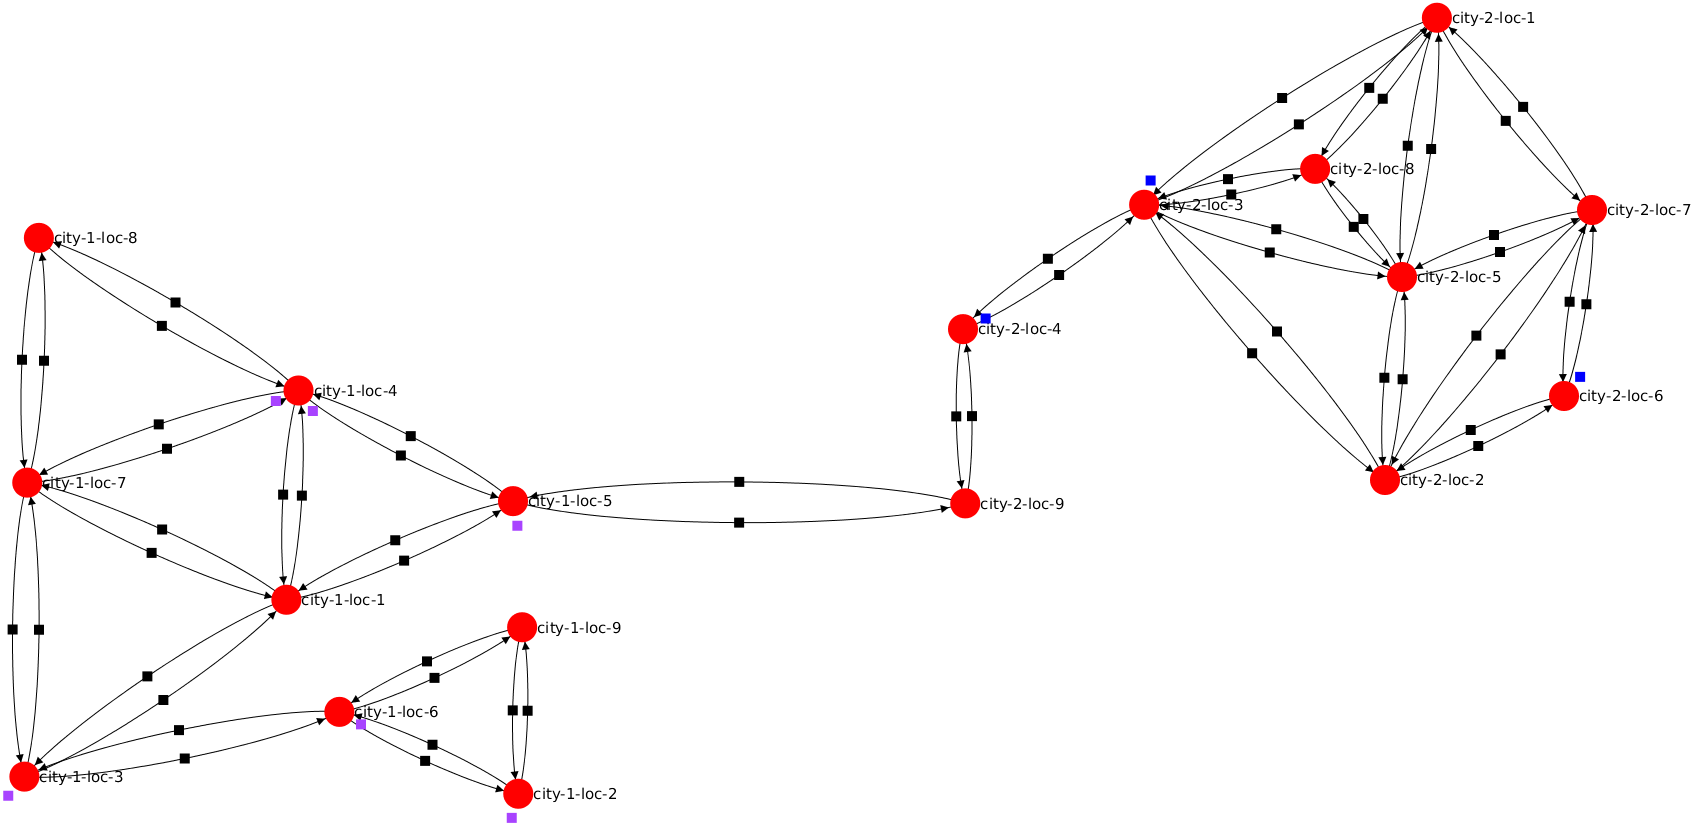
\includegraphics[width=1.0\textwidth]{../img/ipc08_seq-sat_p13_land2}
\end{center}
\caption[Visualization of the \texttt{p13} problem of sequential Transport from IPC 2008.]{Road graph visualization of the \texttt{p13} problem of the seq-sat track of IPC 2008. Red dots represent locations (graph nodes), roads (graph edges) are represented by black arrows, vehicles are plotted as blue squares, and packages as purple squares.}
\label{fig:ipc08_seq-sat_p13}
\end{figure}

\subsection{Transport Numeric}\label{transport-numeric}

The numeric variant adds the concept of fuel on top of the STRIPS variant.
All roads have an additional cost, called \verb+fuel-demand+, which is
subtracted from a vehicle's \verb+fuel-left+ value if it chooses to drive along that road.
Additionally, all vehicles have a maximum fuel capacity \verb+fuel-max+,
which they regain upon being the target of a \verb+refuel+ action. This action can only
be executed at a location that is marked as having a petrol station. Petrol stations
are static with respect to a given planning problem instance.

This variant is usually denoted as \textit{Transport numeric} or \textit{transport-numeric}.

\subsection{Transport Temporal}\label{transport-temporal}

The temporal Transport domain is usually denoted as \textit{Transport temporal} or, confusingly,
also \textit{transport-numeric}. A major difference with respect to the numeric variant is
the addition of time. All actions now have a duration (\verb+pick-up+ and \verb+drop+ both have a
duration of 1, \verb+refuel+ has a duration of 10, and the duration of \verb+drive+ is
equal to the length of the road we are driving along). Furthermore, packages can now have any integral size.

The addition of time poses numerous technical complications when formalizing this variant
--- its PDDL (Section~\ref{pddl}) formulation significantly differs from the two previous ones, but only in technical details, not in objectives of the model.
One important technicality is that a vehicle cannot pick up or drop packages concurrently --- it always handles packages one at a time. Also, vehicles cannot do other actions during driving to another location (they are essentially placed ``off the graph'' for the duration of driving).

The overall goal remains largely the same (deliver packages to their destinations), but we no longer optimize the total cost. Instead, we now minimize the total duration of a plan,
defined as the maximum time when an action is still taking place.
In practice, this translates to minimizing maximum end time over all actions, which is often referred to as minimizing the \textit{makespan}.



















\section{Formalizing the Transport domain}

We will now translate the informal description of the Transport domain from the previous section to the formal representations we defined in Section~\ref{classical-planning}. We will not formulate all the domain variants in all representations as
they are very much alike and not needed for the comprehension of the following chapters.

\subsection{Transport's classical representation}\label{transport-classical-representation}

We are now able to show the sequential Transport domain in one of the representations
previously defined, namely,
the classical representation (Figure~\ref{code:classical-strips}).
For practical reasons, we will use a slight modification, obtained by adding a limited concept of functions
with finite integer values.
It is obvious that we could substitute these functions for the appropriate relations
and a finite amount of literals for the numbers for any given problem instance of
the domain in this representation,
so that it adheres to the definition of a classical formulation.
For example, we could add literals representing a finite set of
natural numbers and a predicate that represents
a successor relation, defined as $\texttt{successor}(a, b) \equiv a + 1 = b$.

Note that this representation does not contain the notion of a \textit{total cost}
of a plan that we will optimize for later.
The predicates used are:
\begin{itemize}
\item \verb+at(o, l)+, the package or vehicle \verb+o+ is at the
location \verb+l+;
\item \verb+capacity(v, s)+, the vehicle \verb+v+ currently has \verb+s+ free space --- \verb+s+ is a variable for space literals, a set of literals denoting the amount of space (essentially,
these literals are a unary representation of a finite set of integers);
\item \verb+capacity-predecessor(s1, s2)+, the space literals represented by \verb+s1+ and \verb+s2+
satisfy the relation $\texttt{s1} + 1 = \texttt{s2}$
in the unary representation;
\item \verb+in(p, v)+, the package \verb+p+ is in the vehicle \verb+v+;
\item \verb+road(l1, l2)+, the location \verb+l1+ is directly adjacent to the location
\verb+l2+ by a road; and
\item \verb+road-length(l1, l2)+, the driving distance between location \verb+l1+
and \verb+l2+, modeled as a numerical function. Does not change while planning.
\end{itemize}

\begin{figure}[tbp]
\begin{code}
drive(v, l1, l2)
  ;; vehicle v moves from location l1 to an adjacent location l2
  precond: at(v, l1), road(l1, l2)
  effects: not at(v, l1), at(v, l2)

pick-up(v, l, p, s1, s2)
  ;; vehicle v picks up package p at location l,
  ;; decreasing its capacity from s2 to s1
  precond: at(v, l), at(p, l), capacity-predecessor(s1, s2),
           capacity(v, s2)
  effects: not at(p, l), in(p, v), capacity(v, s1),
           not capacity(v, s2)
  
drop(v, l, p, s1, s2)
  ;; vehicle v drops package p at location l,
  ;; increasing its capacity from s1 to s2
  precond: at(v, l), in(p, v), capacity-predecessor(s1, s2),
           capacity(v, s1)
  effects: not in(p, v), at(p, l), capacity(v, s2),
           not capacity(v, s1)
\end{code}
\caption{Classical formulation of \texttt{transport-strips}.}
\label{code:classical-strips}
\end{figure}

The numeric variant  adds the \verb+refuel+ operator, changes the \verb+drive+
operator, and adds a new fuel-related predicate \verb+has-petrol-station(l)+, that is true when the given location \verb+l+ has
a petrol station.
To model fuel, we need the addition of a few functions, namely:

\begin{itemize}
\item \verb+fuel-demand(l1, l2)+, the amount of fuel needed to drive
from location \verb+l1+ to location \verb+l2+;
\item \verb+fuel-left(v)+, the amount of fuel left in
the vehicle \verb+v+; and
\item \verb+fuel-max(v)+, the maximum amount of fuel
the vehicle \verb+v+ can contain, i.e. its fuel tank capacity.
\end{itemize}



We also abuse the notation with \verb+decrease+ and \verb+assign+;
the left parameter's value is to be decreased by the right
parameter's value or the left parameter's value is to be overridden
by the right parameter's value, respectively.

See Figure~\ref{code:classical-numeric} for the exact differences
in the representation after adding fuel.

\begin{figure}[tbp]
\begin{code}
drive(v, l1, l2)
  ;; vehicle v moves from location l1 to an adjacent location l2
  precond: at(v, l1), road(l1, l2), fuel-left(v) >= fuel-demand(l1, l2)
  effects: not at(v, l1), at(v, l2),
           decrease(fuel-left(v),  fuel-demand(l1, l2))
  
refuel(v, l)
  ;; vehicle v is refueled to the maximum at location l
  precond: at(v, l), has-petrol-station(l)
  effects: assign(fuel-left(v), fuel-max(v))
\end{code}
\caption[Partial classical formulation of \texttt{transport-numeric}.]{Classical formulation of \texttt{transport-numeric}'s differences compared to \texttt{transport-strips}.}
\label{code:classical-numeric}
\end{figure}

\subsection{Transport's state-variable representation}

We are now also able to show the sequential Transport domain
in the state-variable representation (Figure~\ref{code:statevar-strips}).
Some predicates (\verb+at+, \verb+capacity+ and \verb+in+) have been transformed
into state-variable functions with largely the same semantics as in
Section~\ref{transport-classical-representation}. Again, we leave out
the \textit{total cost} notion.

\begin{figure}[tbp]
\begin{code}
drive(v, l1, l2)
  ;; vehicle v moves from location l1 to an adjacent location l2
  precond: at(v) = l1, road(l1, l2)
  effects: at(v) <- l2

pick-up(v, l, p, s1, s2)
  ;; vehicle v picks up package p at location l,
  ;; decreasing its capacity from s2 to s1
  precond: at(v) = l, at(p) = l, s1 + 1 = s2, s2 > 0, capacity(v) = s2
  effects: at(p) <- nil, in(p) <- v, capacity(v) <- s1
  
drop(v, l, p, s1, s2)
  ;; vehicle v drops package p at location l,
  ;; increasing its capacity from s1 to s2
  precond: at(v) = l, in(p) = v, s1 = s2 - 1, capacity(v) = s1
  effects: in(p) <- nil, at(p) <- l, capacity(v) <- s2
\end{code}
\caption{State-variable formulation of \texttt{transport-strips}.}
\label{code:statevar-strips}
\end{figure}

The numeric variant again adds the \verb+refuel+ operator along with
a few fuel-related state-variable functions and predicates, and changes 
the \verb+drive+ operator (Figure~\ref{code:statevar-numeric}).

\begin{figure}[tb]
\begin{code}
drive(v, l1, l2)
  ;; vehicle v moves from location l1 to an adjacent location l2
  precond: at(v) = l1, road(l1, l2),
           fuel-left(v) >= fuel-demand(l1, l2)
  effects: at(v) <- l2, 
           fuel-left(v) <- fuel-left(v) - fuel-demand(l1, l2)
  
refuel(v, l)
  ;; vehicle v is refueled to the maximum at location l
  precond: at(v) = l, has-petrol-station(l)
  effects: fuel-left(v) <- fuel-max(v)
\end{code}
\caption[Partial state-variable formulation of \texttt{transport-numeric}.]{State-variable formulation of \texttt{transport-numeric}'s differences
compared to \texttt{transport-strips}.}
\label{code:statevar-numeric}
\end{figure}

We will represent the temporal variant of Transport using a variant of the state-variable representation using temporal planning operators, further referred to as the \textit{temporal state-variable representation}.
On top of the fuel-related predicates and functions from \verb+transport-numeric+, temporal Transport adds:
\begin{itemize}
\item \verb+package-size(p)+, a function with positive integer values representing the size of the package \verb+p+ (does not change during planning); and
\item \verb+ready-loading(v)+, a predicate used for ``locking'' the vehicle \verb+v+ during \pickup{} and \drop{} actions (enforcing the property of these two actions happening sequentially in time for a given vehicle). It is important to note that the \refuel{} action does not
lock the vehicle, which means the vehicle can be refueled while dropping off and picking up packages.
\end{itemize}
Figure~\ref{code:statevar-temporal} shows the temporal state-variable representation of Transport temporal, using a shorter but clear notation.

\begin{figure}[tb]
\begin{code}
drive(v, l1, l2)
  ;; vehicle v moves from location l1 to an adjacent location l2
  duration: road-length(l1, l2)
  cond: (at(v) = l1)@s, (road(l1, l2))@s,
        (fuel-left(v) >= fuel-demand(l1, l2))@s
  effects: (at(v) <- nil)@s, (at(v) <- l2)@e,
           (fuel-left(v) <- fuel-left(v) - fuel-demand(l1, l2))@s

pick-up(v, l, p)
  ;; vehicle v picks up package p at location l
  duration: 1
  cond: (at(v) = l1)@[s, e), (at(p) = l1)@s, (ready-loading(v))@s,
        (capacity(v) >= package-size(p))@s
  effects: (at(p) <- nil)@s, (in(p) <- v)@e, (not ready-loading(v))@s,
           (capacity(v) <- capacity(v) - package-size(p))@s,
           (ready-loading(v))@e
  
drop(v, l, p)
  ;; vehicle v drops package p at location l
  duration: 1
  cond: (at(v) = l1)@[s, e), (in(p) = v)@s, (ready-loading(v))@s
  effects: (in(p) <- nil)@s, (at(p) <- l)@e, (not ready-loading(v))@s,
           (capacity(v) <- capacity(v) + package-size(p))@e,
           (ready-loading(v))@e
  
refuel(v, l)
  ;; vehicle v is refueled to the maximum at location l
  duration: 10
  cond: (at(v) = l1)@[s, e), (has-petrol-station(l))@s
  effects: (fuel-left(v) <- fuel-max(v))@e
\end{code}
\caption[State-variable formulation of temporal Transport.]{Temporal state-variable formulation of temporal Transport. The characters \texttt{s} and \texttt{e} represent the start and end temporal variables of the given action, respectively.}
\label{code:statevar-temporal}
\end{figure}

\subsection{PDDL formulation of Transport}

All formulations of the Transport domain use PDDL (Section~\ref{pddl}) version 2.1,
with the requirement \verb+typing+, which adds the notion of types for individual
literals. We will call these literals \textit{action objects}.

The STRIPS variant additionally needs \verb+action-costs+, a requirement adding
integer costs to individual planning operators. These costs may be constant
(like the ones for \verb+pick-up+, \verb+drop+ or \verb+refuel+),
or they may be dependent on the parameters of the instantiated operator (like
the cost of \verb+drive+).
The numeric variant
requires \verb+numeric-fluents+, which introduces native PDDL support for functions whose values correspond to numbers and can change over time. It also requires are
\verb+goal-utilities+, used for custom optimization functions and optional goal predicates.
The temporal domain is similar in requirements to the numeric one, except for
substituting \verb+goal-utilities+ for \verb+durative-actions+ (introduces time
and the duration of actions).
For reference, we will now show the PDDL representation of the sequential and temporal variant of
the Transport domain in Figure~\ref{code:pddl-strips} and Figure~\ref{code:pddl-temporal} respectively.

\begin{figure}[tbp]
\begin{code}
(:action drive
  :parameters (?v - vehicle ?l1 ?l2 - location)
  :precondition (and
      (at ?v ?l1)
      (road ?l1 ?l2))
  :effect (and
      (not (at ?v ?l1))
      (at ?v ?l2)
      (increase (total-cost) (road-length ?l1 ?l2))))
(:action pick-up
  :parameters (?v - vehicle ?l - location ?p - package
               ?s1 ?s2 - capacity-number)
  :precondition (and
      (at ?v ?l)
      (at ?p ?l)
      (capacity-predecessor ?s1 ?s2)
      (capacity ?v ?s2))
  :effect (and
      (not (at ?p ?l))
      (in ?p ?v)
      (capacity ?v ?s1)
      (not (capacity ?v ?s2))
      (increase (total-cost) 1)))
(:action drop
  :parameters (?v - vehicle ?l - location ?p - package
               ?s1 ?s2 - capacity-number)
  :precondition (and
      (at ?v ?l)
      (in ?p ?v)
      (capacity-predecessor ?s1 ?s2)
      (capacity ?v ?s1))
  :effect (and
      (not (in ?p ?v))
      (at ?p ?l)
      (capacity ?v ?s2)
      (not (capacity ?v ?s1))
      (increase (total-cost) 1)))
\end{code}
\caption{Formulation of actions in PDDL for \texttt{transport-strips}.}
\label{code:pddl-strips}
\end{figure}

\begin{figure}[tbp]
\begin{code}
(:durative-action drive
  :parameters (?v - vehicle ?l1 ?l2 - location)
  :duration (= ?duration (road-length ?l1 ?l2))
  :condition (and
      (at start (at ?v ?l1))
      (at start (road ?l1 ?l2))
      (at start (>= (fuel-left ?v) (fuel-demand ?l1 ?l2))))
  :effect (and
      (at start (not (at ?v ?l1)))
      (at end (at ?v ?l2))
      (at start (decrease (fuel-left ?v) (fuel-demand ?l1 ?l2)))))
(:durative-action pick-up
  :parameters (?v - vehicle ?l - location ?p - package)
  :duration (= ?duration 1)
  :condition (and
      (at start (at ?v ?l))
      (over all (at ?v ?l))
      (at start (at ?p ?l))
      (at start (>= (capacity ?v) (package-size ?p)))
      (at start (ready-loading ?v)))
  :effect (and
      (at start (not (at ?p ?l)))
      (at end (in ?p ?v))
      (at start (decrease (capacity ?v) (package-size ?p)))
      (at start (not (ready-loading ?v))) ; lock vehicle
      (at end (ready-loading ?v)))) ; unlock vehicle
(:durative-action drop
  :parameters (?v - vehicle ?l - location ?p - package)
  :duration (= ?duration 1)
  :condition (and
      (at start (at ?v ?l))
      (over all (at ?v ?l))   
      (at start (in ?p ?v))
      (at start (ready-loading ?v)))
  :effect (and (at start (not (in ?p ?v)))
      (at end (at ?p ?l))
      (at end (increase (capacity ?v) (package-size ?p)))
      (at start (not (ready-loading ?v))) ; lock vehicle
      (at end (ready-loading ?v)))) ; unlock vehicle
(:durative-action refuel
  :parameters (?v - vehicle ?l - location)
  :duration (= ?duration 10)
  :condition (and
      (at start (at ?v ?l))
      (over all (at ?v ?l))
      (at start (has-petrol-station ?l)))
  :effect
      (at end (assign (fuel-left ?v) (fuel-max ?v))))
\end{code}
\caption{Formulation of durative actions in PDDL for temporal Transport.}
\label{code:pddl-temporal}
\end{figure}
















\section{Related problems}

To the best of our knowledge, there has been no attempt at producing domain-dependent planners
for Transport (IPC 2008, 2011, 2014 and unsolvability IPC 2016) or any other similar IPC domain, like Logistics (IPC 1998\comment{\footnote{\url{https://web.archive.org/web/20151017170331/http://ipc98.icaps-conference.org/}}} and 2000),
Depots (IPC 2002\comment{\footnote{\url{https://web.archive.org/web/20170408120817/http://ipc02.icaps-conference.org/domains.html}}}),
DriverLog (IPC 2002 and 2014),
or Trucks (IPC 2006).
All techniques we know of applied to Transport so far are the
domain-independent planners used in the three before-mentioned competitions.

Most of the research done on transportation-related problems and their automation
generally focuses
on a famous combinatorial optimization problem, the \textit{Traveling Salesman Problem} (TSP), on which an
exhaustive amount of research has been done \citep{Applegate1998, Applegate2011}. Its precise origins are unknown, but the problem has been on the minds of researchers at least since the end of the 19$^\textrm{th}$ century. The TSP is defined by \citet{Applegate2011} as follows:
\begin{quote}
Given a set of cities along with the cost of travel between each pair of them, the \textit{traveling salesman problem}, or \textit{TSP} for short, is to find the cheapest way of visiting all the cities and returning to the starting point. The ``way of visiting all the cities'' is simply the order in which the cities are visited; the ordering is called a \textit{tour} or \textit{circuit} through the cities.
\end{quote}
However, the problem we aim to study is more similar to a different optimization problem based on the TSP. See Figure~\ref{fig:tsp} for an illustrative example of a TSP solution.

\begin{figure}[tbp]
\begin{center}
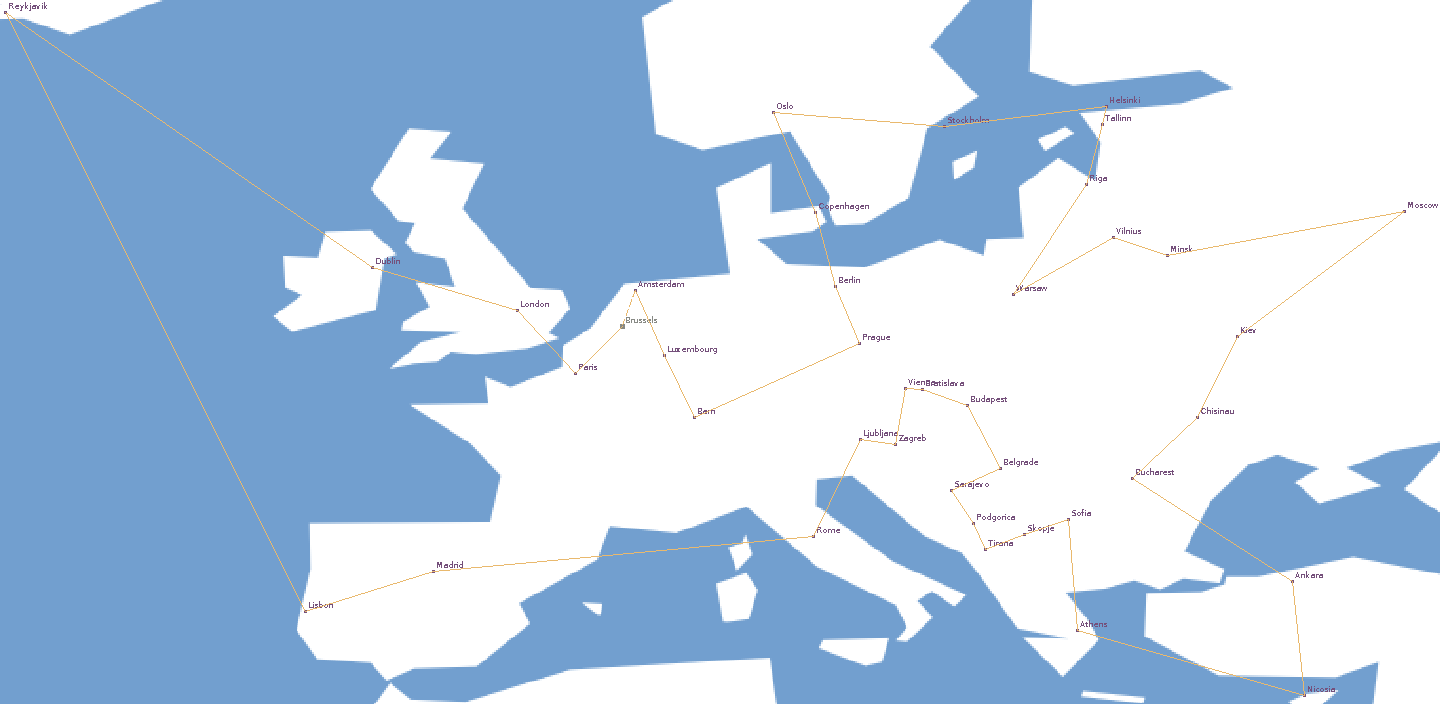
\includegraphics[width=1.0\textwidth]{../img/tsp}
\end{center}
\caption[An example TSP solution through the capitals of Europe.]{An example TSP solution through the capitals of Europe. Screenshot taken from OptaPlanner \citep{DeSmet2017}.}
\label{fig:tsp}
\end{figure}

\subsection{The Vehicle Routing Problem}\label{vrp}

The \textit{Vehicle Routing Problem} (VRP) was first formulated as the \textit{Truck Dispatching Problem} by \citet{Dantzig1959}, modeling a fleet of vehicles delivering gasoline to service stations. They described VRP
as a generalization of the TSP with multiple vehicles, but it could equivalently be stated that the TSP is a specialization of the VRP
with a single vehicle. The precise formulation of the Truck Dispatching Problem in \citep[Section~2]{Dantzig1959} represents a model with a fleet of identical vehicles departing from a single depot. According to \citet[Section~3]{Braekers2016}, this defines what we would call \textit{Capacitated VRP} (CVRP) today (Figure~\ref{fig:vrp}).

\begin{figure}[tbp]
\begin{center}
\includegraphics[width=0.7\textwidth]{../img/vrp}
\end{center}
\caption[An example CVRP solution for 32 customers and one depot.]{An example CVRP solution for 32 customers and one depot. Screenshot taken from OptaPlanner \citep{DeSmet2017}.}
\label{fig:vrp}
\end{figure}

Many VRP variants have emerged since. \citet{Eksioglu2009} and \citet{Braekers2016} both
review and classify hundreds of papers related to the VRP, with many more left out.
Most of these works tend to study the CVRP problem with minor modifications, hence creating
a broad landscape of problems and a platform to build on for the future.
According to the data in \citet[Table~4]{Braekers2016}, there has been a recent uptick
in popularity for models relatively similar to Transport --- specifically, VRPs with
backhauls (returning items from customers to depots),
multiple depots (multiple starting points for vehicles), and with allowed split deliveries (multiple
vehicles can serve a single customer).
The literature review on multiple depot VRP (MDVRP) in \citet{Montoya-Torres2015}
suggests a big rise in popularity for MDVRP in the recent past,
which provides further proof of relevance for studying the Transport domain.

Traditional solutions for the VRP include exact approaches like branch and bound
or constraint satisfaction
programming
that explore the large parts of the feasible search space,
classical heuristics which limit the search space, and also metaheuristics (general heuristics for devising specific heuristics), like genetic algorithms, local search, tabu search, and many more.

\comment{
\subsection{VRP Formulation}\citep{ResearchGroup2013}

The VRP is a combinatorial problem whose ground set is the edges of a graph ${G(V,E)}$. The notation used for this problem is as follows:

\begin{itemize}
\item ${V = \left\lbrace v_{0}, v_{1}, \ldots, v_{n} \right\rbrace}$ is a vertex set, where:
\begin{itemize}
\item Consider a depot to be located at ${v_0}$.
\item Let ${V' = V \backslash \left\lbrace v_{0} \right\rbrace}$ be used as the set of ${n}$ cities.
\end{itemize}
\item ${A = \left\lbrace(v_{i},v_{j}) | v_{i},v_{j} \in V; i \neq j \right\rbrace}$ is an arc set.
\item ${C}$ is a matrix of non-negative costs or distances ${c_{ij}}$ between customers ${v_{i}}$ and ${v_{j}}$.
\item ${d}$ is a vector of the customer demands.
\item ${R_{i}}$ is the route for vehicle ${i}$.
\item ${m}$ is the number of vehicles (all identical). One route is assigned to each vehicle.
\end{itemize}

When $c_{ij} = c_{ji}$ for all $(v_{i}, v_{j}) \in A$ the problem is said to be symmetric and it is then common to replace ${A}$ with the edge set $E = \lbrace (v_{i},v_{j}) | v_{i},v_{j} \in V; i < j \rbrace$.

With each vertex ${v_{i}}$ in ${V'}$ is associated a quantity ${q_{i}}$ of some goods to be delivered by a vehicle. The VRP thus consists of determining a set of ${m}$ vehicle routes of minimal total cost, starting and ending at a depot, such that every vertex in ${V'}$ is visited exactly once by one vehicle.

For easy computation, it can be defined ${b(V) = \left\lceil \sum_{v_{i} \in V} d_{i}) / C \right\rceil}$, an obvious lower bound on the number of trucks needed to service the customers in set ${V}$.

We will consider a service time $\delta_{i}$ (time needed to unload all goods), required by a vehicle to unload the quantity ${q_{i}}$ at ${v_{i}}$. It is required that the total duration of any vehicle route (travel plus service times) may not surpass a given bound ${D}$, so, in this context the cost ${c_{ij}}$ is taken to be the travel time between the cities. The VRP defined above is NP-hard [Lenstra \& Rinnooy Kan 1981].

A feasible solution is composed of:

\begin{itemize}
\item a partition ${R_{1}, \ldots, R_{m}}$ of ${V}$;
\item a permutation ${\sigma_{i}}$ of ${R_{i} \bigcup {0}}$ specifying the order of the customers on route ${i}$.
\end{itemize}


The cost of a given route (${R_{i} = \left\lbrace v_{0}, v_{1}, \ldots, v_{m+1} \right\rbrace}$), where ${v_{i} \in V}$ and ${v_{0} = v_{m+1} = 0}$ (0 denotes the depot), is given by ${C(R_{i}) = \sum_{i=0}^{m} c_{i,i+1} + \sum_{i=1}^{m} \delta_{i}}$.

A route ${R_{i}}$ is feasible if the vehicle stop exactly once in each customer and the total duration of the route does not exceed a prespecified bound ${D}$: ${C(R_{i}) \leq D}$.

Finally, the cost of the problem solution ${S}$ is: ${F_{VRP} = \sum_{i=1}^{m} F(R_{i})}$.
}

\subsection{Comparison of Transport and VRP}

In \citet{ResearchGroup2013}, a website was created, which serves as a comprehensive resource on the history of VRP,
definitions of its various flavors, and an overview of the popular solution methods and state-of-the-art results. According to the taxonomy they propose, we could characterize a Transport domain problem
as a \textit{Multiple Depot, Split Delivery, Capacitated VRP with Satellite Facilities}. Multiple Depot
means that vehicles can start driving from multiple locations, split delivery
means a single customer can be served by multiple vehicles, capacitated VRP adds maximum
capacities to vehicles, and satellite facilities mean that vehicles can pick items up
while on a delivery route. This does not characterize the Transport domain in every detail, but it is a fairly accurate approximation.

According to another VRP taxonomy and study of papers, presented in \citet{Eksioglu2009} and adapted in \citet{Braekers2016}, no research has been done on a VRP variant with a similar subset of features to those of Transport in any single study, to the best of our knowledge.
Usually, the studied problems are more constrained than Transport --- for example, they make additional assumptions about the places where vehicles start or end. Also, VRP in general
makes cooperation of vehicles hard to model, whereas in Transport this is one of the fundamental elements.

\comment{Transport could be characterized as \textit{2.1.1, 2.2.1, 2.4.1, 2.5.1, 2.8.1, 3.1.1, 3.2.2, 3.3.3, 3.4.2, 3.5.2, 3.7.1, 3.8.1, 3.9.3, 3.10.1, 3.11.1, 4.1.1, 4.2.1, 4.3.2, 4.4.1, 5.1.2.}}

An important difference between Transport and the VRP is that Transport has a notion of single packages or items. In the VRP, transported goods are usually regarded as measurable, rather than countable (for example gasoline or milk vs. letters or parcels). This makes a difference not only in the
interpretation, but also during problem-solving --- \textit{customers} in VRP usually request
a quantity of the delivered item, not specific item instances, like packages being ``requested''
by their target locations in Transport.
